\section{Results and discussion}
\subsection{Optimalisation of the classifier parameters}
By performing a five fould crossvalidation during the trainingstage the most
optimal parameterset for the RF algorithm was searched for.  It was found that
for all levels except the first, a value of 5 yields optimal results for the
parameter minimum samples per leaf. For level 1, this optimal value was
significantly higher at 55. %TODO why?

For each level of the classifier a threshold was set to determine which voxels
would be allowed to the next level (i.e. which voxels showed a high nodule
probability). In order to avoid discarding nodulevoxels of rather small nodules
a rather low threshold had to be set. It was empirically set at 0,1 for all
levels except for the last one. At the final level a treshold of 0,9 was set to
determine which voxels would be taken into account into our final list of
detected nodules.
 
\subsection{Validation results}
The obtained sensitivity of the algorithm was 100\% with an average of 2,17 TP
per scan and an average of 1787 FP per scan. %accuracy
% TODO mss duidelijk als je scans bekijkt welke FP zijn? TODO FPs of FP?
The algorithm shows to perform well concerning the detection of the nodules, but
by setting the thresholds at a higher value the amount of FP will probably be
reduced. Due to a lack of time the optimal thresholds were not determined
anymore. Another improvement that could be made is training the algorithm on
more datasets. To determine the optimal amount of datasets a comparison should
be made between the time it takes to train the algorithm on a certain amount of
scans and the improvements that are obtained in the performances of the
algorithm by increasing the amount of scans.

Although comparing the performances of different studies in a meaningful way is
rather difficult due to the reasons mentioned before in \ref{sec:performance}.
\cite{teramoto} showed a sensitivity of 80\% and 4,2 FP per LIDC/IDRI scan.
The detection speed was 25-34 seconds per scan. This study performed a FP reduction
by using a SVM classifier. \cite{elbaz} showed a sensitivity of 82,3\% and a
specificity of 9,2\%. The time to process 1 scan was about 5 minutes.
\cite{ginneken} compared the performances of six nodule detection CAD algorithms
on the same validation dataset. The sensitivities at seven levels of false
positive detection were calculated and then averaged. The best performing method
in this study yielded an average sensitivity of 63,2\% for the detection of all
kinds of nodules. The sensitivity per nodule type was also provided: small
nodules (63,4\%), large nodules (62,8\%), isolated nodules (60,9\%), vascular
nodules (69,3\%), pleural nodules (43,5\%) and peri-fissural nodules (76,6\%).
This clearly shows that the ease of nodule detection also depends on the type of
nodule. As this information is not available in the annotations of the scans and
as we did not cooperate with a radiologist, it is not possible to differentiate
between the different types of nodules in this project. However, as we may
assume that different nodule types are represented in our testset, it is clear
the algorithm is able to detect several types of nodules except for extremely
small ones as we removed these from the annotations in the training and
validation phase.


\begin{figure}[ht]
\begin{center}
	\begin{subfigure}[b]{\linewidth}
		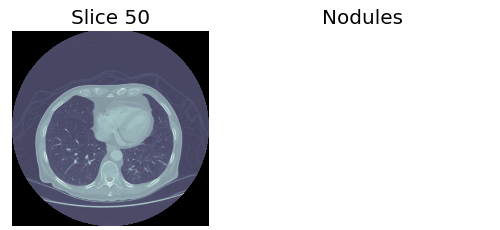
\includegraphics[width=\linewidth]{img/cascades/D50S50.png}
		\caption{Slice 50}
	\end{subfigure}
	\begin{subfigure}[b]{\linewidth}
		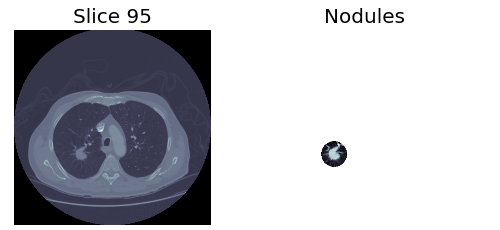
\includegraphics[width=\linewidth]{img/cascades/D50S95.png}
  		\caption{Slice 95}
	\end{subfigure}
	\caption{Example of two slices in dataset 50, one without and one with a
	nodule.}
	\label{fig:d50}
\end{center}
\end{figure}

\begin{figure*}[p] %TODO add percentage start/left, bigger threshold at end
\begin{center}
	\begin{subfigure}[b]{0.5\linewidth}
		\begin{subfigure}[b]{\linewidth}
			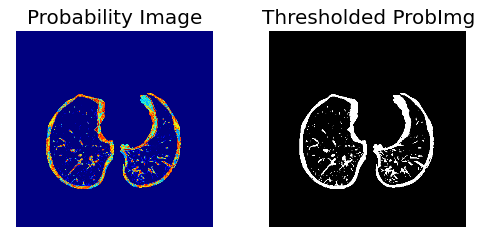
\includegraphics[width=\linewidth]{img/cascades/D50L1S50.png}
			\caption{Level 1 -- Threshold: xx\% -- xx\% remaining}
		\end{subfigure}
		\begin{subfigure}[b]{\linewidth}
			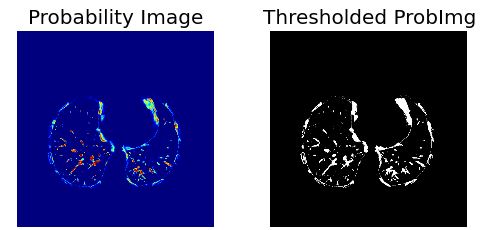
\includegraphics[width=\linewidth]{img/cascades/D50L2S50.png}
			\caption{Level 2 -- Threshold: xx\% -- xx\% remaining}
		\end{subfigure}
		\begin{subfigure}[b]{\linewidth}
			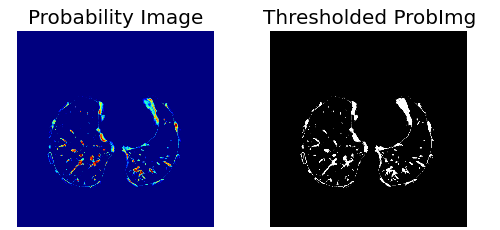
\includegraphics[width=\linewidth]{img/cascades/D50L3S50.png}
			\caption{Level 3 -- Threshold: xx\% -- xx\% remaining}
		\end{subfigure}
		\begin{subfigure}[b]{\linewidth}
			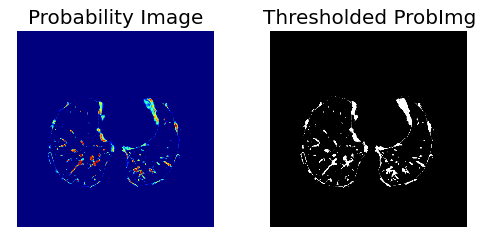
\includegraphics[width=\linewidth]{img/cascades/D50L4S50.png}
			\caption{Level 4 -- Threshold: xx\% -- xx\% remaining}
		\end{subfigure}
	  \caption{Processed versions of slice 50 in dataset 50. Left: probability
	  image. Right: threshold of probability image showing the voxels that continue
	  to the next level in the cascade.}
	  \label{fig:d50s50}
  \end{subfigure}
  \begin{subfigure}[b]{0.5\linewidth}
  		\begin{subfigure}[b]{\linewidth}
			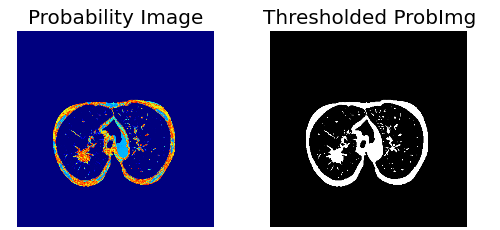
\includegraphics[width=\linewidth]{img/cascades/D50L1S95.png}
			\caption{Level 1}
		\end{subfigure}
		\begin{subfigure}[b]{\linewidth}
			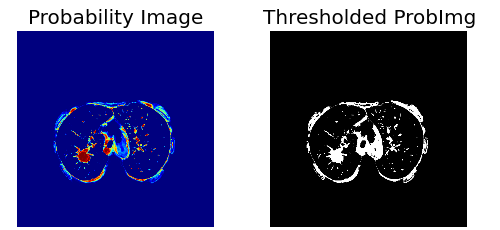
\includegraphics[width=\linewidth]{img/cascades/D50L2S95.png}
			\caption{Level 2}
		\end{subfigure}
		\begin{subfigure}[b]{\linewidth}
			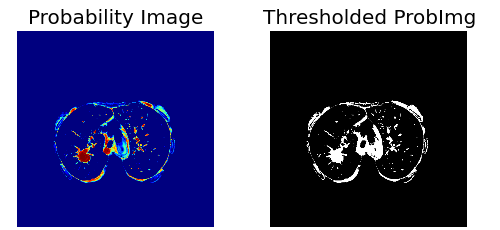
\includegraphics[width=\linewidth]{img/cascades/D50L3S95.png}
			\caption{Level 3}
		\end{subfigure}
		\begin{subfigure}[b]{\linewidth}
			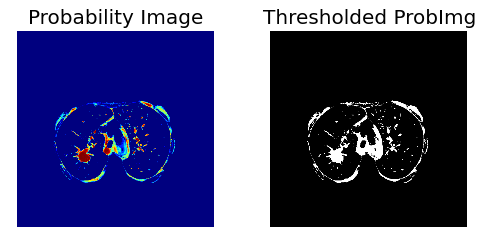
\includegraphics[width=\linewidth]{img/cascades/D50L4S95.png}
			\caption{Level 4}
		\end{subfigure}
	  \caption{Processed versions of slice 95 in dataset 50. Left: probability
	  image. Right: threshold of probability image showing the voxels that continue
	  to the next level in the cascade. The same thresholds and remaining counts
	  apply as in figure \ref{fig:d50s50}.}
	  \label{fig:d50s95}
  \end{subfigure}
\end{center}
\end{figure*}

% \begin{figure}[p]
% \begin{center}
% 	\begin{subfigure}[b]{\linewidth}
% 		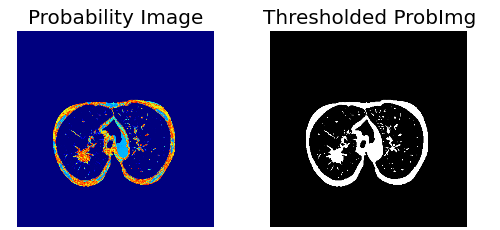
\includegraphics[width=\linewidth]{img/cascades/D50L1S95.png}
% 		\caption{Level 1}
% 	\end{subfigure}
% 	\begin{subfigure}[b]{\linewidth}
% 		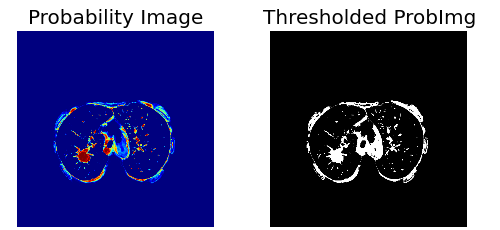
\includegraphics[width=\linewidth]{img/cascades/D50L2S95.png}
% 		\caption{Level 2}
% 	\end{subfigure}
% 	\begin{subfigure}[b]{\linewidth}
% 		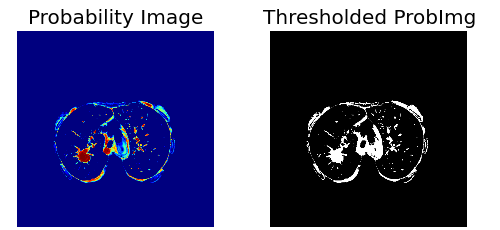
\includegraphics[width=\linewidth]{img/cascades/D50L3S95.png}
% 		\caption{Level 3}
% 	\end{subfigure}
% 	\begin{subfigure}[b]{\linewidth}
% 		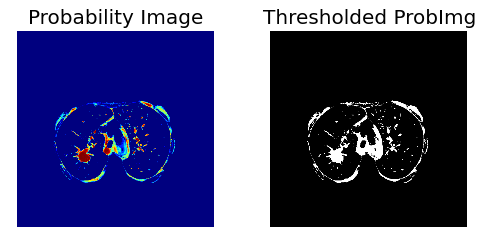
\includegraphics[width=\linewidth]{img/cascades/D50L4S95.png}
% 		\caption{Level 4}
% 	\end{subfigure}
%   \caption{Processed versions of slice 95 in dataset 50. Left: probability
%   image. Right: threshold of probability image showing the voxels that continue
%   to the next level in the cascade. The same thresholds and remaining counts
%   apply as in figure \ref{fig:d50s50}.}
%   \label{fig:d50s95}
% \end{center}
% \end{figure}

\subsection{Suggestions for improvements}
% TODO However, the annotations assign a probability of malignancy for each
% nodule.
Separating the detected nodules into a malignancy or benignancy class is not the
main aim of this project, but this might be implemented as an extra feature.
In the ideal case, the algorithm would be able to do the processing in a couple
of minutes. This would be very interesting for a commercial software product.
However, considering the available computational power (a laptop) and the
scripting language that is used, this would not be feasible. Python is an
interpreted language which makes it inherently slower than compiled languages
such as C++. Nevertheless, Python was chosen for its rapid prototyping
abilities. Future work may implement our algorithm in C++ or another compiled
language to speed up the computational process.




